\documentclass[11pt,compress,t,notes=noshow, xcolor=table]{beamer}
\usepackage[]{graphicx}\usepackage[]{color}
% maxwidth is the original width if it is less than linewidth
% otherwise use linewidth (to make sure the graphics do not exceed the margin)
\makeatletter
\def\maxwidth{ %
  \ifdim\Gin@nat@width>\linewidth
    \linewidth
  \else
    \Gin@nat@width
  \fi
}
\makeatother

\newcommand{\citebutton}[2]{%
\beamergotobutton{\href{#2}{#1}}%
}

\newcommand{\blu}[1]{\textcolor{blue}{#1}}
\newcommand{\org}[1]{\textcolor{orange}{#1}}
\newcommand{\ques}{\textbf{\textcolor{red}{Question:  }}}
\newcommand{\questionssofar}{\begin{frame}\frametitle{Any questions?}\end{frame}}

\newcommand\warning{%
 \makebox[1.4em][c]{%
 \makebox[0pt][c]{\raisebox{.1em}{\scriptsize!}}%
 \makebox[0pt][c]{\color{red}\normalsize$\bigtriangleup$}}}%

\definecolor{fgcolor}{rgb}{0.345, 0.345, 0.345}
\newcommand{\hlnum}[1]{\textcolor[rgb]{0.686,0.059,0.569}{#1}}%
\newcommand{\hlstr}[1]{\textcolor[rgb]{0.192,0.494,0.8}{#1}}%
\newcommand{\hlcom}[1]{\textcolor[rgb]{0.678,0.584,0.686}{\textit{#1}}}%
\newcommand{\hlopt}[1]{\textcolor[rgb]{0,0,0}{#1}}%
\newcommand{\hlstd}[1]{\textcolor[rgb]{0.345,0.345,0.345}{#1}}%
\newcommand{\hlkwa}[1]{\textcolor[rgb]{0.161,0.373,0.58}{\textbf{#1}}}%
\newcommand{\hlkwb}[1]{\textcolor[rgb]{0.69,0.353,0.396}{#1}}%
\newcommand{\hlkwc}[1]{\textcolor[rgb]{0.333,0.667,0.333}{#1}}%
\newcommand{\hlkwd}[1]{\textcolor[rgb]{0.737,0.353,0.396}{\textbf{#1}}}%
\let\hlipl\hlkwb

\usepackage{framed}
\makeatletter
\newenvironment{kframe}{%
 \def\at@end@of@kframe{}%
 \ifinner\ifhmode%
  \def\at@end@of@kframe{\end{minipage}}%
  \begin{minipage}{\columnwidth}%
 \fi\fi%
 \def\FrameCommand##1{\hskip\@totalleftmargin \hskip-\fboxsep
 \colorbox{shadecolor}{##1}\hskip-\fboxsep
     % There is no \\@totalrightmargin, so:
     \hskip-\linewidth \hskip-\@totalleftmargin \hskip\columnwidth}%
 \MakeFramed {\advance\hsize-\width
   \@totalleftmargin\z@ \linewidth\hsize
   \@setminipage}}%
 {\par\unskip\endMakeFramed%
 \at@end@of@kframe}
\makeatother

\definecolor{shadecolor}{rgb}{.97, .97, .97}
\definecolor{messagecolor}{rgb}{0, 0, 0}
\definecolor{warningcolor}{rgb}{1, 0, 1}
\definecolor{errorcolor}{rgb}{1, 0, 0}
\newenvironment{knitrout}{}{} % an empty environment to be redefined in TeX

\usepackage{alltt}
\newcommand{\SweaveOpts}[1]{}  % do not interfere with LaTeX
\newcommand{\SweaveInput}[1]{} % because they are not real TeX commands
\newcommand{\Sexpr}[1]{}       % will only be parsed by R
\newcommand{\xmark}{\ding{55}}%


\usepackage[english]{babel}
\usepackage[utf8]{inputenc}

\usepackage{dsfont}
\usepackage{verbatim}
\usepackage{amsmath}
\usepackage{amsfonts}
\usepackage{amssymb}
\usepackage{bm}
\usepackage{csquotes}
\usepackage{multirow}
\usepackage{longtable}
\usepackage{booktabs}
\usepackage{enumerate}
\usepackage[absolute,overlay]{textpos}
\usepackage{psfrag}
\usepackage{algorithm}
\usepackage{algpseudocode}
\usepackage{eqnarray}
\usepackage{arydshln}
\usepackage{tabularx}
\usepackage{placeins}
\usepackage{tikz}
\usepackage{setspace}
\usepackage{colortbl}
\usepackage{mathtools}
\usepackage{wrapfig}
\usepackage{bm}
\usepackage{amsmath}
\usepackage{pifont}

\usetikzlibrary{shapes.multipart,shapes,arrows,automata,positioning,calc,chains,trees, shadows}
\tikzset{
  %Define standard arrow tip
  >=stealth',
  %Define style for boxes
  punkt/.style={
    rectangle,
    rounded corners,
    draw=black, very thick,
    text width=6.5em,
    minimum height=2em,
    text centered},
  % Define arrow style
  pil/.style={
    ->,
    thick,
    shorten <=2pt,
    shorten >=2pt,}
}

\tikzstyle{vec}=[draw, rectangle, fill = white, minimum width=5mm, minimum height=1cm, inner sep = 2pt]

\usepackage{subfig}

% Defines macros and environments
\usepackage{../../style/lmu-lecture}


\let\code=\texttt
\let\proglang=\textsf

\setkeys{Gin}{width=0.9\textwidth}

\setbeamertemplate{frametitle}{\expandafter\uppercase\expandafter\insertframetitle}

\usepackage{bbm}
% basic latex stuff
\newcommand{\pkg}[1]{{\fontseries{b}\selectfont #1}} %fontstyle for R packages
\newcommand{\lz}{\vspace{0.5cm}} %vertical space
\newcommand{\dlz}{\vspace{1cm}} %double vertical space
\newcommand{\oneliner}[1] % Oneliner for important statements
{\begin{block}{}\begin{center}\begin{Large}#1\end{Large}\end{center}\end{block}}


%new environments
\newenvironment{vbframe}  %frame with breaks and verbatim
{
 \begin{frame}[containsverbatim,allowframebreaks]
}
{
\end{frame}
}

\newenvironment{vframe}  %frame with verbatim without breaks (to avoid numbering one slided frames)
{
 \begin{frame}[containsverbatim]
}
{
\end{frame}
}

\newenvironment{blocki}[1]   % itemize block
{
 \begin{block}{#1}\begin{itemize}
}
{
\end{itemize}\end{block}
}

\newenvironment{fragileframe}[2]{  %fragile frame with framebreaks
\begin{frame}[allowframebreaks, fragile, environment = fragileframe]
\frametitle{#1}
#2}
{\end{frame}}


\newcommand{\myframe}[2]{  %short for frame with framebreaks
\begin{frame}[allowframebreaks]
\frametitle{#1}
#2
\end{frame}}

\newcommand{\remark}[1]{
  \textbf{Remark:} #1
}


\newenvironment{deleteframe}
{
\begingroup
\usebackgroundtemplate{
\includegraphics[width=\paperwidth,height=\paperheight]{../style/color/red.png}}
 \begin{frame}
}
{
\end{frame}
\endgroup
}
\newenvironment{simplifyframe}
{
\begingroup
\usebackgroundtemplate{
\includegraphics[width=\paperwidth,height=\paperheight]{../style/color/yellow.png}}
 \begin{frame}
}
{
\end{frame}
\endgroup
}\newenvironment{draftframe}
{
\begingroup
\usebackgroundtemplate{
\includegraphics[width=\paperwidth,height=\paperheight]{../style/color/green.jpg}}
 \begin{frame}
}
{
\end{frame}
\endgroup
}
% https://tex.stackexchange.com/a/261480: textcolor that works in mathmode
\makeatletter
\renewcommand*{\@textcolor}[3]{%
  \protect\leavevmode
  \begingroup
    \color#1{#2}#3%
  \endgroup
}
\makeatother





\input{../../latex-math/basic-math.tex}
\input{../../latex-math/basic-ml.tex}

\newcommand{\titlefigure}{figure/ml-basics-supervised-classif-task.png}
\newcommand{\learninggoals}{
\item Know definition and examples of supervised tasks
\item Understand the difference between regression and classification}

\title{Introduction to Machine Learning}
% \author{Bernd Bischl, Christoph Molnar, Daniel Schalk, Fabian Scheipl}
\institute{\href{https://compstat-lmu.github.io/lecture_i2ml/}{compstat-lmu.github.io/lecture\_i2ml}}
\date{}

\begin{document}


\lecturechapter{ML-Basics: Supervised Tasks}
\lecture{Introduction to Machine Learning}

% ------------------------------------------------------------------------------

\begin{vbframe}{Tasks: Regression vs Classification}

\begin{itemize}
    \item Supervised tasks are data situations where learning the functional
        relationship between inputs (features) and output (target) is
        useful.
    
    \item The two most basic tasks are 
        regression and classification, depending on whether the 
        target is numerical or categorical.
\end{itemize}  

\lz

\begin{columns}    
\begin{column}{0.5\textwidth} 
\textbf{Regression}: Our observed labels come from $\Yspace \in \mathbb{R}$.

  \begin{center}
    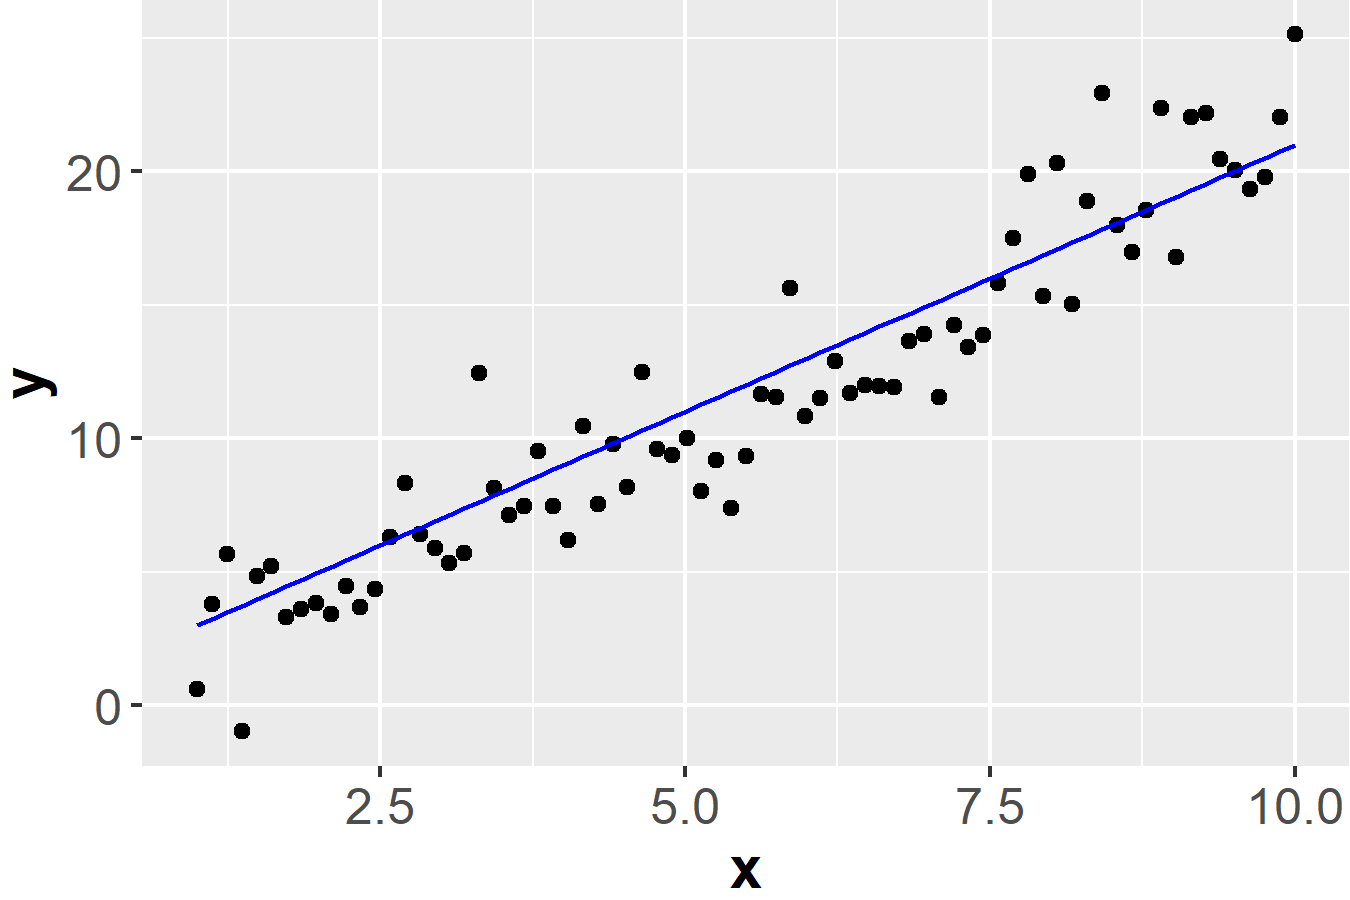
\includegraphics[width=\textwidth]{figure/ml-basics-supervised-regression-task.png} 
  \end{center}
\end{column}    

\begin{column}{0.5\textwidth} 
\textbf{Classification}: Observations are categorized: $y \in \Yspace = \{C_1,...,C_g\}$.
  
  \begin{center}
    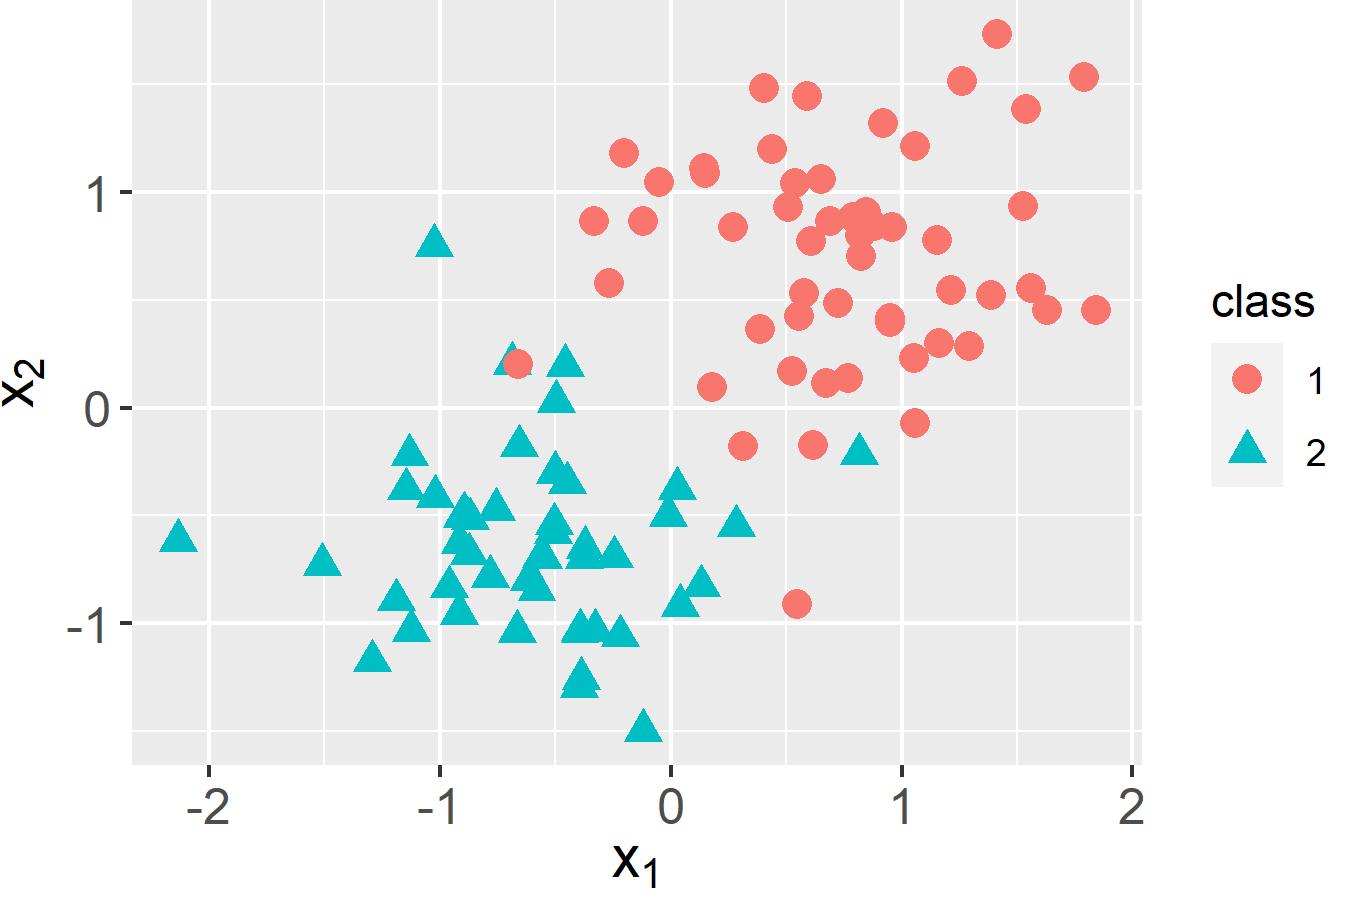
\includegraphics[width=\textwidth]{figure/ml-basics-supervised-classif-task.png} 
  \end{center}
\end{column}    
\end{columns}    
  
\end{vbframe}

\begin{vbframe}{Predict vs. Explain}
We can distinguish two main reasons to learn this relationship:


\begin{itemize}
    \item \textbf{Learning to predict}. In such a case we potentially do not care how
        our model is structured or whether we can understand it.\\
        Example: predicting how a stock price will develop. \\
        Simply being able to use the predictor on new data is of direct benefit to us.

    \item \textbf{Learning to explain}. Here, our model is only a means to 
        a better understanding of the inherent relationship in the data.\\
        Example: understanding which risk factors influence the probability to 
        get a certain disease.
        We might not use the learned model on new observations, but rather 
        discuss its implications, in a scientific or social context.

\end{itemize}  

While ML was traditionally more interested in the former, classical statistics
addressed the latter. In many tasks nowadays both are relevant -- to different degrees.

\end{vbframe}
  
  
% \end{itemize}  

% \framebreak

% \begin{itemize}

  % \item The set-up in supervised learning will typically look like this:
  % 
  % \begin{itemize}
  % 
  %   \item We restrict our options to a certain class of functions,
  %   
  %   \item choose some metric to evaluate model candidates,
  %   
  %   \item and try to find the best candidate in an efficient way.
  %   
  % \end{itemize} 
  % 
  % \item This procedure is carried out by an algorithm called \textbf{learner} or
  % \textbf{inducer}.
  


\begin{vbframe}{Regression example: House Prices}

%\begin{enumerate}

  %\item 
  Predict the price for a house in a certain area
    
    
    \begin{center}
    %https://docs.google.com/presentation/d/1m86-HK5-iCWbWpc_ssm2sZBQ8yxexIfjKcQXDU6DWss/edit?usp=sharing page 1
    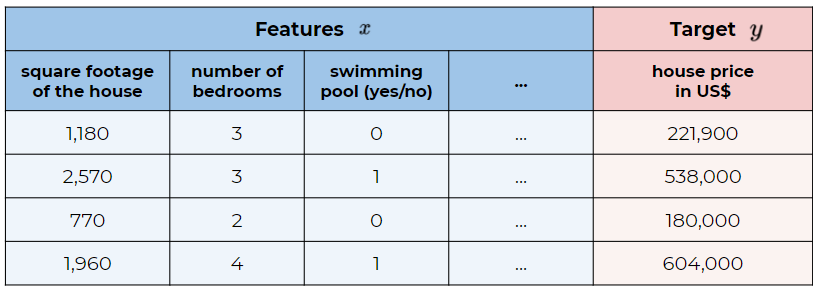
\includegraphics[width=0.5\textwidth]{figure_man/ml-basics-supervised-task-houses-data.png} 
    
    \lz
    
    %https://unsplash.com/photos/sPpe2D7VbpM
    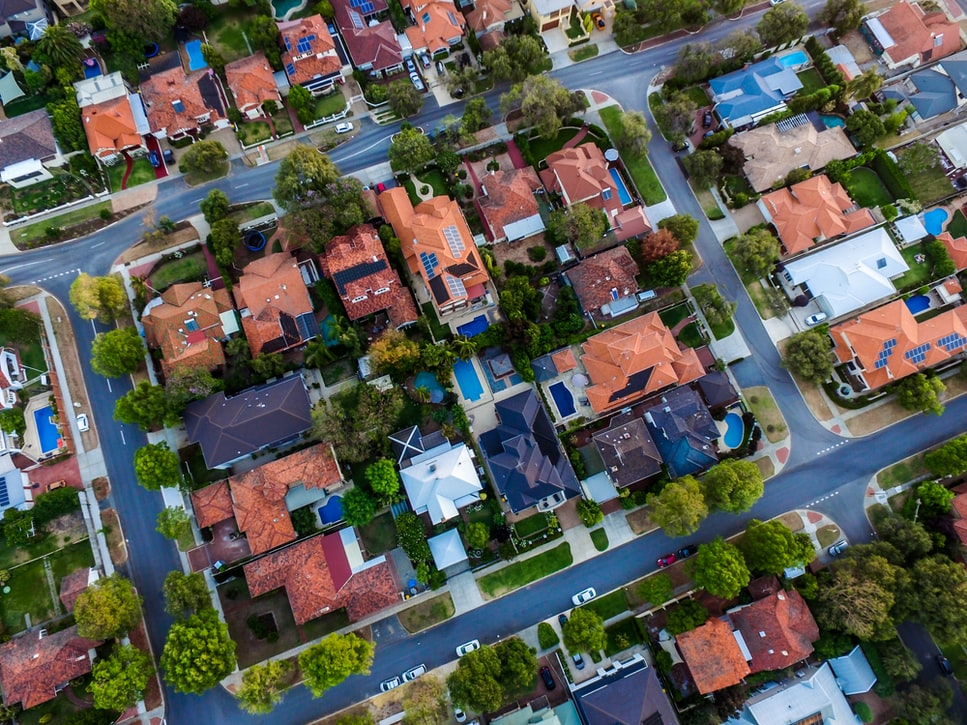
\includegraphics[width=0.3\textwidth]{figure_man/ml-basics-supervised-task-houses-pic.jpg} 
    
    \end{center}

    Probably \textit{learn to explain}. We might want to understand what influences 
    a house price most. But maybe we are also looking for underpriced houses and
    the predictor is of direct use, too.
    
%\end{enumerate}

\end{vbframe}

%------------------

\begin{vbframe}{Regression example: Length-of-stay}
  
  Predict days a patient has to stay in hospital at time of admission
       
    
    \begin{center}
    %https://docs.google.com/presentation/d/1m86-HK5-iCWbWpc_ssm2sZBQ8yxexIfjKcQXDU6DWss/edit?usp=sharing page 2
    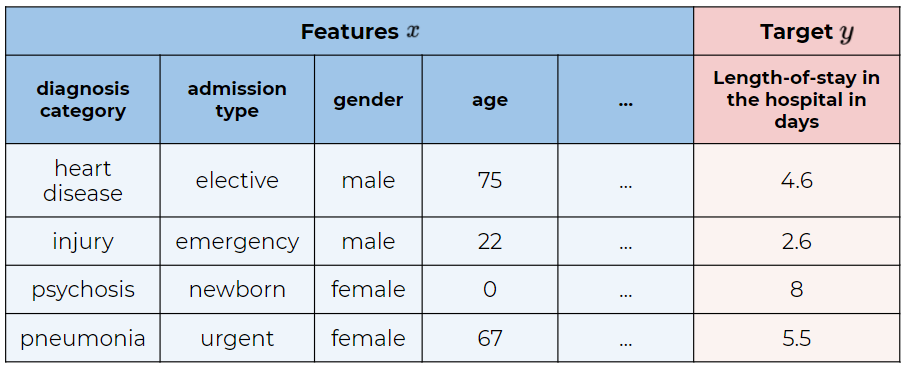
\includegraphics[width=0.6\textwidth]{figure_man/ml-basics-supervised-task-hosp-data.png} 
    
    \lz
    
    %https://unsplash.com/photos/ZCO_5Y29s8k
    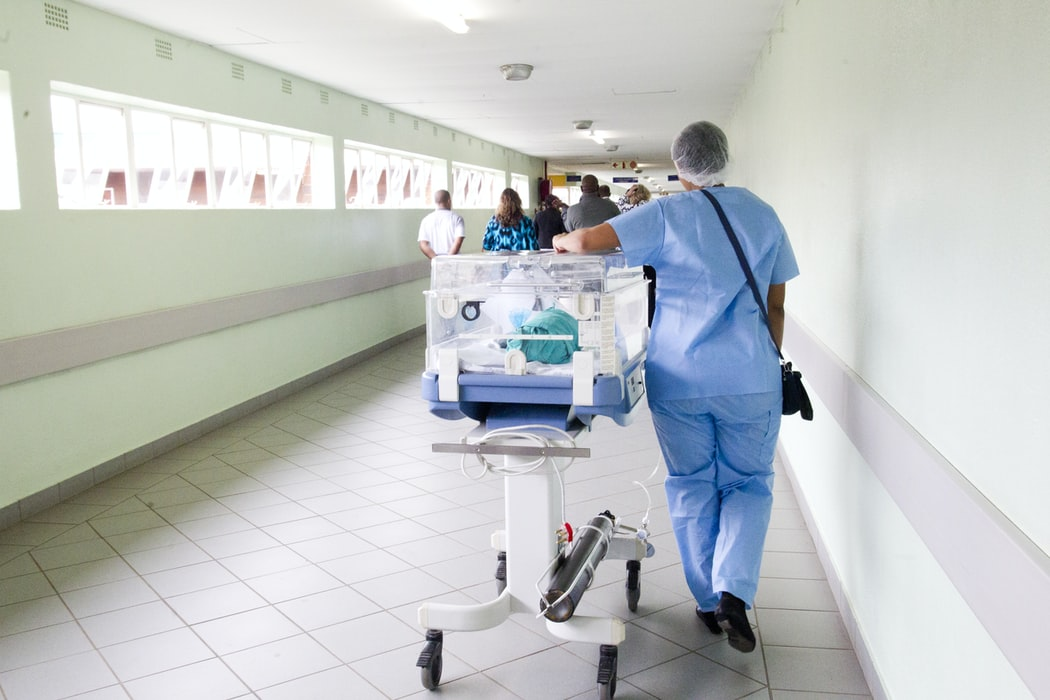
\includegraphics[width=0.3\textwidth]{figure_man/ml-basics-supervised-task-hosp-pic.jpg} 
    
    \end{center}
    
    Can be \textit{learn to explain}, but \textit{learn to predict} would help
    a hospital's planning immensely. 
  
  
%\end{enumerate}

\end{vbframe}

% ------------------------------------------------------------------------------

\begin{vbframe}{Classification example: Risk category}

  Predict one of five risk categories for a life insurance customer to determine the insurance premium 
\begin{center}

   %https://docs.google.com/presentation/d/1m86-HK5-iCWbWpc_ssm2sZBQ8yxexIfjKcQXDU6DWss/edit?usp=sharing page 3
    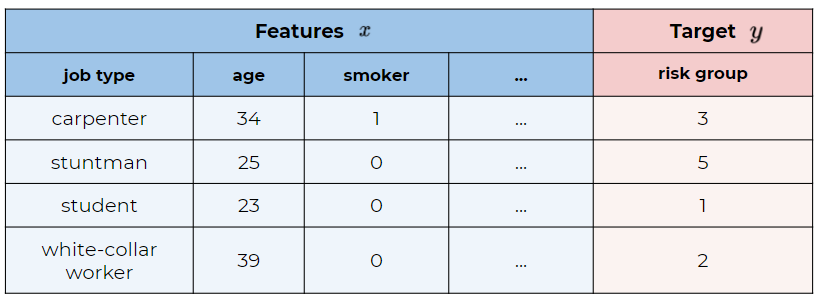
\includegraphics[width=0.5\textwidth]{figure_man/ml-basics-supervised-task-insurance-data.png} 

\lz

% FIGURE SOURCE: https://docs.google.com/presentation/d/1WLPubv9vxLL-JIlHAtsvTBBG5pbF4xgRGW_prkOAEnE/edit?usp=sharing Page 3
  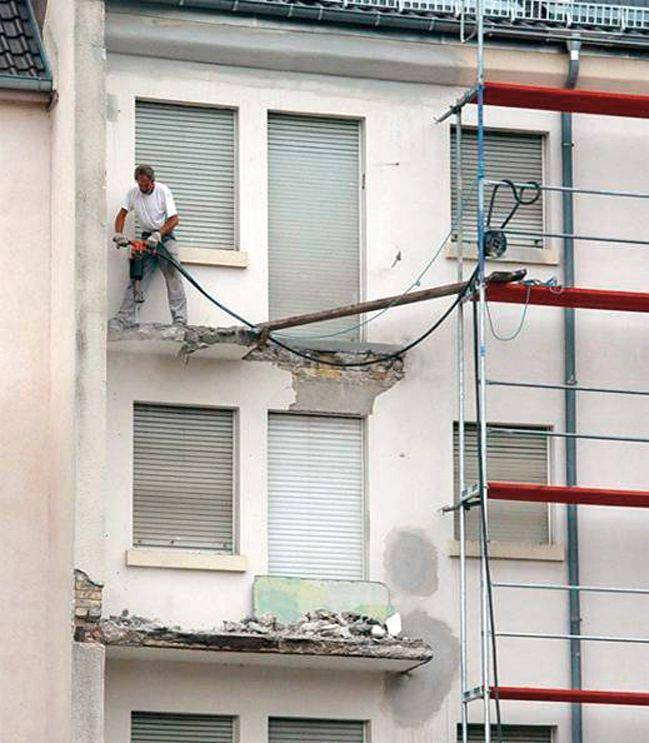
\includegraphics[width = 0.2\textwidth]{figure_man/classif_ex_placeholder.jpg} 
\end{center}

Probably \textit{learn to predict}, but the company might be required to explain
its predictions to its customers.

\end{vbframe}

%%%%%%%%%%hierhin


% ------------------------------------------------------------------------------

% \begin{vbframe}{Supervised Learning}
% 
% \begin{itemize}
% 
%   \item \textbf{Supervised} learning means we make use of \emph{labeled}
%   data, i.e., observations for which we already know the target outcome.
%   
%   \item We try to construct $f$ automatically from an example set of such 
%   labeled objects.
%   
%   \item Using the thus learned model, we can make \textbf{predictions} based on
%   the features of our data.
% 
%   \item Knowing the \enquote{truth} allows us to test how well we have grasped 
%   the nature of the underlying mapping by comparing our predictions to the 
%   actually observed values.
%   
% \end{itemize} 
% 
% \end{vbframe}




% ------------------------------------------------------------------------------


% -----------------------------------------------------------------------------

% ------------------------------------------------------------------------------

% \begin{vbframe}{Summary}
% 
% \medskip
% 
% \textbf{Supervised machine learning} is concerned with learning a function 
% that predicts a certain \textbf{target} from an object's \textbf{features} 
% from a set of examples for which both the features and the target are known.\\
% The function to be learned is restricted to come from a certain class of 
% functions and its precise shape is defined in terms of a set of 
% \textbf{parameters}.
% 
% \end{vbframe}

% ------------------------------------------------------------------------------

\endlecture
\end{document}
